
%%%%%%%%%%%%%%%%%%%%%%% file typeinst.tex %%%%%%%%%%%%%%%%%%%%%%%%%
%
% This is the LaTeX source for the instructions to authors using
% the LaTeX document class 'llncs.cls' for contributions to
% the Lecture Notes in Computer Sciences series.
% http://www.springer.com/lncs       Springer Heidelberg 2006/05/04
%
% It may be used as a template for your own input - copy it
% to a new file with a new name and use it as the basis
% for your article.
%
% NB: the document class 'llncs' has its own and detailed documentation, see
% ftp://ftp.springer.de/data/pubftp/pub/tex/latex/llncs/latex2e/llncsdoc.pdf
%
%%%%%%%%%%%%%%%%%%%%%%%%%%%%%%%%%%%%%%%%%%%%%%%%%%%%%%%%%%%%%%%%%%%

% ○ 問題を沢山使ってる例を出す
% わからない問題でもいいことを示す Who's the bully? when?
% ○エピソードを使う認証は多いが、パスワードを生成するものは何故かない
% ○  毎日の行動から認証するものもある
% 家族や友人が知らない秘密は存在するはず
% 秘密の質問が駄目と言われるのは質問の質が悪いから
%
% ○ 拡張機能の説明
%
% ○ 参考文献たくさん
% 大きなことをいわない
% パスワードを覚えるのは無理
% ○ シード文字列の選びかた
% エントロピーの計算
% アルゴリズムの選択 
% 偽答生成が簡単であることを示す 
% サポートシステムを作っていることをかく ★

\documentclass[runningheads,a4paper]{llncs}

\usepackage{amssymb}
\setcounter{tocdepth}{3}
\usepackage{graphicx}
\usepackage{marginnote}

\usepackage{here} % [H]とするとその場所に配置されるらしい

\usepackage{url}
% \urldef{\mailsa}\path|masui@pitecan.com|
\urldef{\mailsa}\path|***@***.***.***|
\newcommand{\keywords}[1]{\par\addvspace\baselineskip
\noindent\keywordname\enspace\ignorespaces#1}

\begin{document}

\mainmatter  % start of an individual contribution

% first the title is needed
\title{EpisoPass: Password Management based on Episodic Memories}

% a short form should be given in case it is too long for the running head
\titlerunning{EpisoPass: Password Management based on Episodic Memories}

% the name(s) of the author(s) follow(s) next
%
% NB: Chinese authors should write their first names(s) in front of
% their surnames. This ensures that the names appear correctly in
% the running heads and the author index.
%
% \author{Toshiyuki Masui%
\author{***** ****
% \thanks{Thanks...}%
}
%
\authorrunning{Lecture Notes in Computer Science: Authors' Instructions}
% (feature abused for this document to repeat the title also on left hand pages)

% the affiliations are given next; don't give your e-mail address
% unless you accept that it will be published
%\institute{Faculty of Environment and Information Studies, Keio University\\
%5322 Endo, Fujisawa, Kanagawa 252-8520, Japan\\
%\mailsa\\
%\url{http://pitecan.com/}}
\institute{******* ******* ******* *******\\
******, ****** *******, *******\\
\mailsa\\
% \url{http://pitecan.com/}}
\url{http://*****.***.***/}}

%
% NB: a more complex sample for affiliations and the mapping to the
% corresponding authors can be found in the file "llncs.dem"
% (search for the string "\mainmatter" where a contribution starts).
% "llncs.dem" accompanies the document class "llncs.cls".
%

\toctitle{Lecture Notes in Computer Science}
\tocauthor{Authors' Instructions}
\maketitle


\begin{abstract}
We propose a password manager \textit{EpisoPass} that supports the
generation of strong passwords based on a user's secret episodic
memories. To use EpisoPass, a user first collects question-answer
pairs related to their own episodic memories. Each is registered with
several possible answers: a single correct answer and multiple fake
answers. When the user wants to generate a password, EpisoPass shows
each question and list of possible answers and asks the user to select
those that are correct. EpisoPass then generates a domain-unique
password by substituting the characters of a seed string based on the
selected answers. Through careful selection of memories and answers,
EpisoPass provides an authentication step using memories that are easy
to recall, but difficult for others to guess. In this way various
strong passwords can be easily managed without the need for the master
password or secret device that is otherwise required by conventional
password managers. Using a browser extension, users can use EpisoPass
directly on the login page of conventional Web services like Facebook,
removing the need to type or copy a password string.

\keywords{Passwords; password managers; user authentication; episodic memories; EpisoPass}
\end{abstract}

\section{Introduction}

Passwords have been used as a means of authenticating to Web services and applications
for a long time, and remain the most popular authentication method on the Internet.
%
Since short passwords are easily guessable by attackers and
using the same password for multiple services is unsafe,
a different long password should be used for each service a person uses.
However, remembering numerous long passwords is almost impossible for ordinary humans.
%
According to research conducted by Flor\^{e}ncio {\it et al.\/} in 2007,
people use on average only 6.5 different passwords to access 25 Web services, and
4.28\% of users forget their passwords within 3 months \cite{Florencio:2007:LSW:1242572.1242661}.

Since passwords are difficult to handle, various other authentication methods have been proposed.
For example, image-based authentication \cite{Biddle:2012:GPL:2333112.2333114,GraphicalPasswords}, 
biometrics\footnote{
  % \textsf{https:{\slash}{\slash}en.wikipedia.org{\slash}wiki{\slash}Biometrics}
  \url{https://en.wikipedia.org/w/index.php?title=Biometrics&oldid=736189000}
},
behavior-based authentication \cite{Dandapat:2015:AYD:2702123.2702457}, and many others.

% というのもパスワードには利点があるから[Bonneau]
%   すでに普及
%   KB以外の特殊ハードが要らない
%   アタック方法はいろいろあるし[] 流出もしばしばだが
%     うまく実装したシステム上でうまく使えば安全
%     ハッシュ、ソルト
%     実装が比較的簡単
% なのでパスワードが近い将来死滅するとは考えられない

% \marginnote{I'd hesitate to call passwords the {\it strongest\/} method. Perhaps {\it most widely deployed\/} would be less contreversial?}
However, password-based authentication is still the most
convenient and widely deployed method \cite{Bonneau:ReplacePasswords},
and is not expected to disappear any time soon \cite{Herley:2009:PSS:1601990.1602010}.

Given we will have to continue to live with password-based authentication systems for the foreseeable future,
we have to devise practical methods for handling many passwords, and various ``password managers'' have been proposed
\cite{OnePassword,Dashlane,MilPass,LastPass,KeyPass,NortonIDSafe,IDManager}.
%
Password managers remember users' passwords and aim to directly enter them into the login pages of the various services a user wants to access.
%
The burden on the user is reduced by requiring just a single ``master password'' to access the database of stored passwords.
%
Although password managers are widely used and a clear step forward from having to remember multiple passwords, uses nonetheless have to remember the master password or use a special hardware device for safely handling the password database, and password managers usually run on only a limited set of devices.

% 読みとることができない脳内情報を利用するという基本手法は良いのだが覚えられないのが問題である
%   だとすると...パスワードを記憶するかわりに、****脳が既に覚えている秘密の記憶からパスワードを生成すればよいはずである***
%   確かな脳内情報を使ってパスワードを利用する必要があるが、
%     沢山の強力なパスワードそのものを覚えることは不可能に近い
%   だとすると、確かな脳内秘密情報からパスワードをGenerateするしかない
%   そこでエピソード記憶を使う
%   秘密の知識からGenerateするとよい
%

If we want to avoid having to carry any special device for authentication,
either we must used some form of biometrics, or all the information required 
for the authentication must be
must be stored in the user's memory.
%
However, the biggest problem with memory-based authentication is that
users cannot reliably remember passwords or master password that are long and complex enough to be secure.
For this reason, we believe that
it is far better to ``generate'' something for the authentication,
based on a user's episodic memories. This has the benefit that unlike a password, a person is highly unlikely to forget such episodic memories.
%
% We believe that a password manager should have the following features.
% (1) It should be available on any platform including PCs, smartphones, and the Web.
% (2) Users should not have secret information (e.g. master password) or special device.
% (3) Rely only on the information in the user's brain.
%
We therefore propose \textit{EpisoPass}, a password manager that generates strong passwords
based only on a user's secret and unforgettable episodic memories.

\section{EpisoPass}

EpisoPass is a password manager that supports the generation of
strong passwords based on a user's secret episodic memories.
%
% Before using EpisoPass for generating passwords,
% a user provides a seed string and many question-answer pairs to EpisoPass,
% and a password is generated based on the user's selections.
%
% Memories in human brain are not uniform.
Our brains store numerous memories, but different memories have different characteristics.
Some memories are very short-lived, while others are recallable for long periods of time.
When we have a particularly impressive experience,
the memory of it will stay in our mind for a long time and can't be easily forgotten.
On the other hand, other topics are more difficult to remember. For example, when studying mathematics and trying to remember a new formula,
it can be hard to memorize without significant practice,
since knowledge of the formula is unrelated to
any personal experiences.
The former type of memory is called an {\it episodic\/} memory and most people find such
memories easy to recollect and hard to forget.
Memories of passwords belong in the latter category. People find them
hard to remember and easy to forget, in the same way people find it difficult
to remember mathematical formulas.

% \begin{quote}
% Episodic memory is the memory of autobiographical events (times,
% places, associated emotions, and other contextual who, what, when,
% where, why knowledge) that can be explicitly stated. It is the
% collection of past personal experiences that occurred at a particular
% time and place. For example, if one remembers the party on his or her
% 6th birthday, this is an episodic memory. They allow an individual to
% figuratively travel back in time to remember the event that took place
% at that particular time and place.[1]
% 
% Semantic memory is one of the two types of declarative or explicit
% memory (our memory of facts or events that is explicitly stored and
% retrieved).[1] Semantic memory refers to general world knowledge that
% we have accumulated throughout our lives.[2] This general knowledge
% (facts, ideas, meaning and concepts) is intertwined in experience and
% dependent on culture. Semantic memory is distinct from episodic
% memory, which is our memory of experiences and specific events that
% occur during our lives, from which we can recreate at any given
% point.[3] For instance, semantic memory might contain information
% about what a cat is, whereas episodic memory might contain a specific
% memory of petting a particular cat. We can learn about new concepts by
% applying our knowledge learned from things in the past.[4] The
% counterpart to declarative, or explicit memory, is procedural memory,
% or implicit memory.[5]
% \end{quote}

\begin{figure}
\centering
% 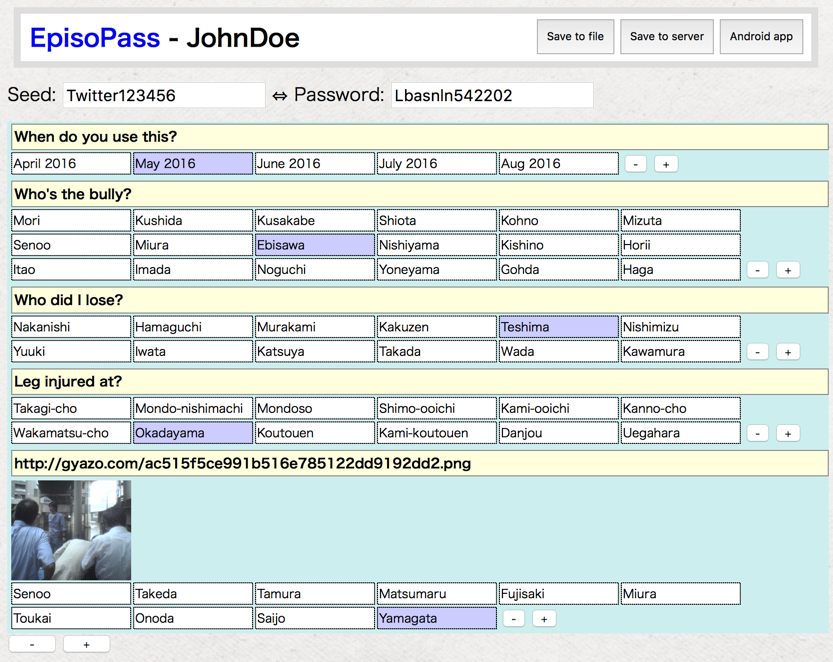
\includegraphics[width=1.0\columnwidth]{figures/c1bd6e7f67698c70978f528ccd2339d9}
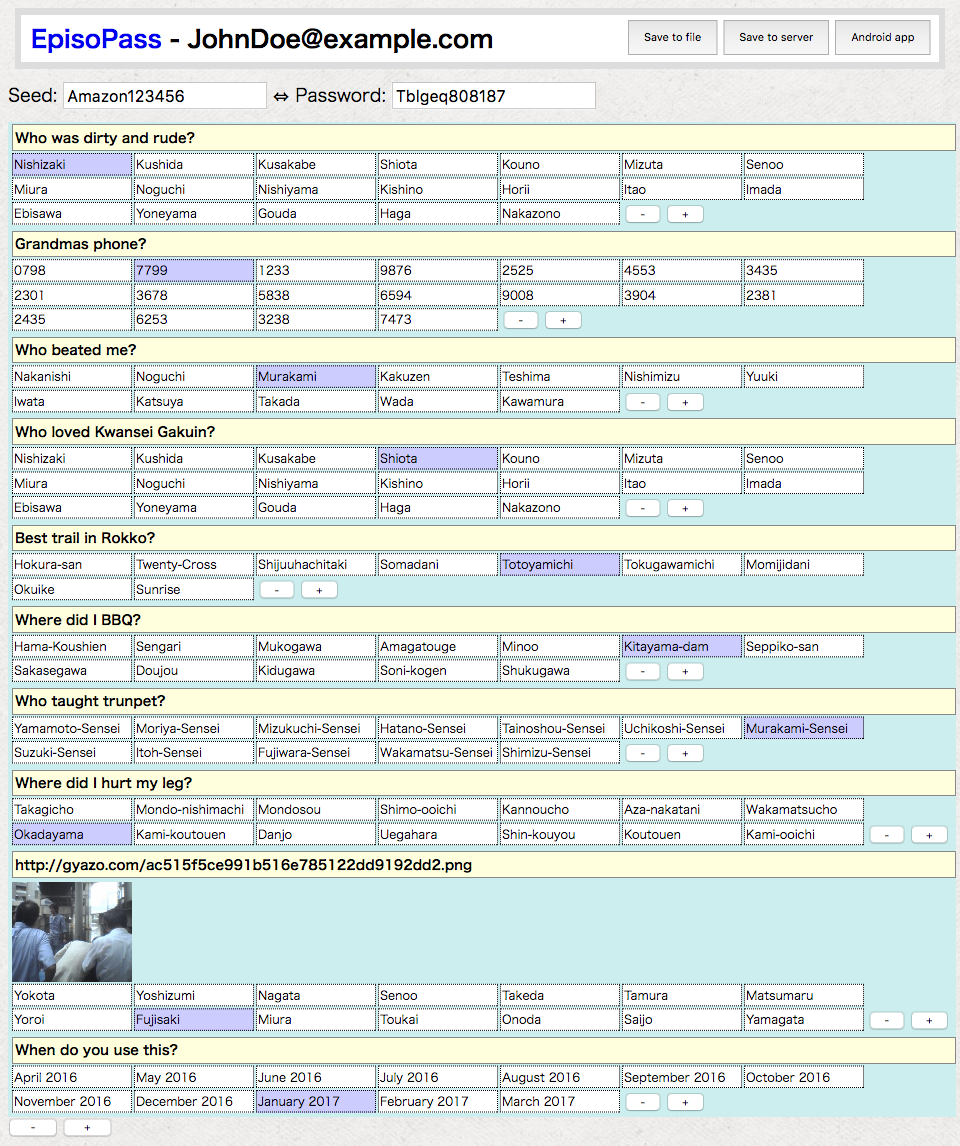
\includegraphics[width=1.0\columnwidth]{figures/4d13e6804ba790624c1f8e2b8255bde5}
\caption{Generating an Amazon password with EpisoPass.}
\label{web1}
\end{figure}

% \marginnote{You mention that episodic memories and cognitive passwords
%   have been used in the past, but it's not clear to me (from the text
%   here) why your system is different. Perhaps you could put a sentence
%   or two about this?}

The idea of using episodic memories for authentication has a long
history and early papers suggested using episodic memories for
creating passwords \cite{Barton:Password}.
Authentication using secret questions is sometimes
referred to as ``cognitive
passwords''\cite{Zviran:1990:UAC:100512.100538}, and such approaches
have been used as an alternative to password-based authentication
systems.
%
While cognitive passwords were aimed to be alternatives to
password-based systems, EpisoPass is a system for supporting
password-based systems using episodic memories.

Password generation on EpisoPass is performed through the following steps:

\begin{enumerate}
\item A user registers multiple question texts related to their own personal
secret unforgettable episodic memories. For each question they must provides
a single correct answer and multiple additional incorrect answers.

\item The user provides a long ``seed string'' for each service that requires
a password.

\item EpisoPass shows the questions and answers to the user allowing
them to select the correct answer for each question.
Based on the user's selections,
EpisoPass substitutes characters in the seed string and generates a
strong password candidate string.
After selecting all of the correct answers,
the user copies the calculated string
and registers it as the password for the service.
\end{enumerate}

\subsection{Using EpisoPass in a browser}

Figure \ref{web1} shows how to generate a password
on EpisoPass running in a browser by accessing the EpisoPass site.
Many questions related to the user's episodic memories are shown to the user,
and many candidate answers are also shown for each question.
When a user clicks and selects one of the answers for a question,
the seed string shown at the top-left is converted to a
candidate password string based on the selections. If incorrect answers are chosen the wrong password will be generated. On the other hand, when the user selects the correct answers for all of the questions,
the correct password is calculated and shown at the top of the page.

% If the q-a is based on the user's episodic memories and
% nobody knows the correct answer,
% only the user can select the set of right answers and
% use the converted string as the password.

In Figure \ref{web1},
``\textsf{Amazon123456}'' is provided as the seed string,
and based on the selections to the ten questions,
the seed string is converted to the string
``\textsf{Tblgeq808187}'',
to be used as the password for Amazon.com.

When the user clicks on different candidate answers 
the seed string is converted to a completely different string, such as
``\textsf{Xvdkzb940345}'', as shown in Figure \ref{web11}.

In this way, different selections yield different password strings and
the unique password string generated after selecting the correct answers should be
used as the password for the service.

% Frank:
% This is a very overconstraining way of saying ``upper, lower and
% digits''. First, it says ``one upper, five lower, six
% digits''. Second, it puts them in specific places. Aren't you being a
% lot more prescriptive than the site's own policy? This reduces the
% space of passwords that can be generated, for very little benefit.
%
% そうかな? まぁ言いたいことはわかるけど

Capital letters in the seed string are substituted for capital letters in the password,
and digits in the seed string are substituted for digits. In this way
the generated password can be arranged to conform with any password character restrictions
the site might impose.

The first question in Figure \ref{web1}
is based on the author's episodic memory at elementary school,
and the question with a photo at the bottom is related to a more recent event
which the author believes he will never forget.
All the questions are based on the author's episodic memories that he's unlikely to ever forget,
and that he believes nobody else will know the correct answer for.

\begin{figure}
\centering
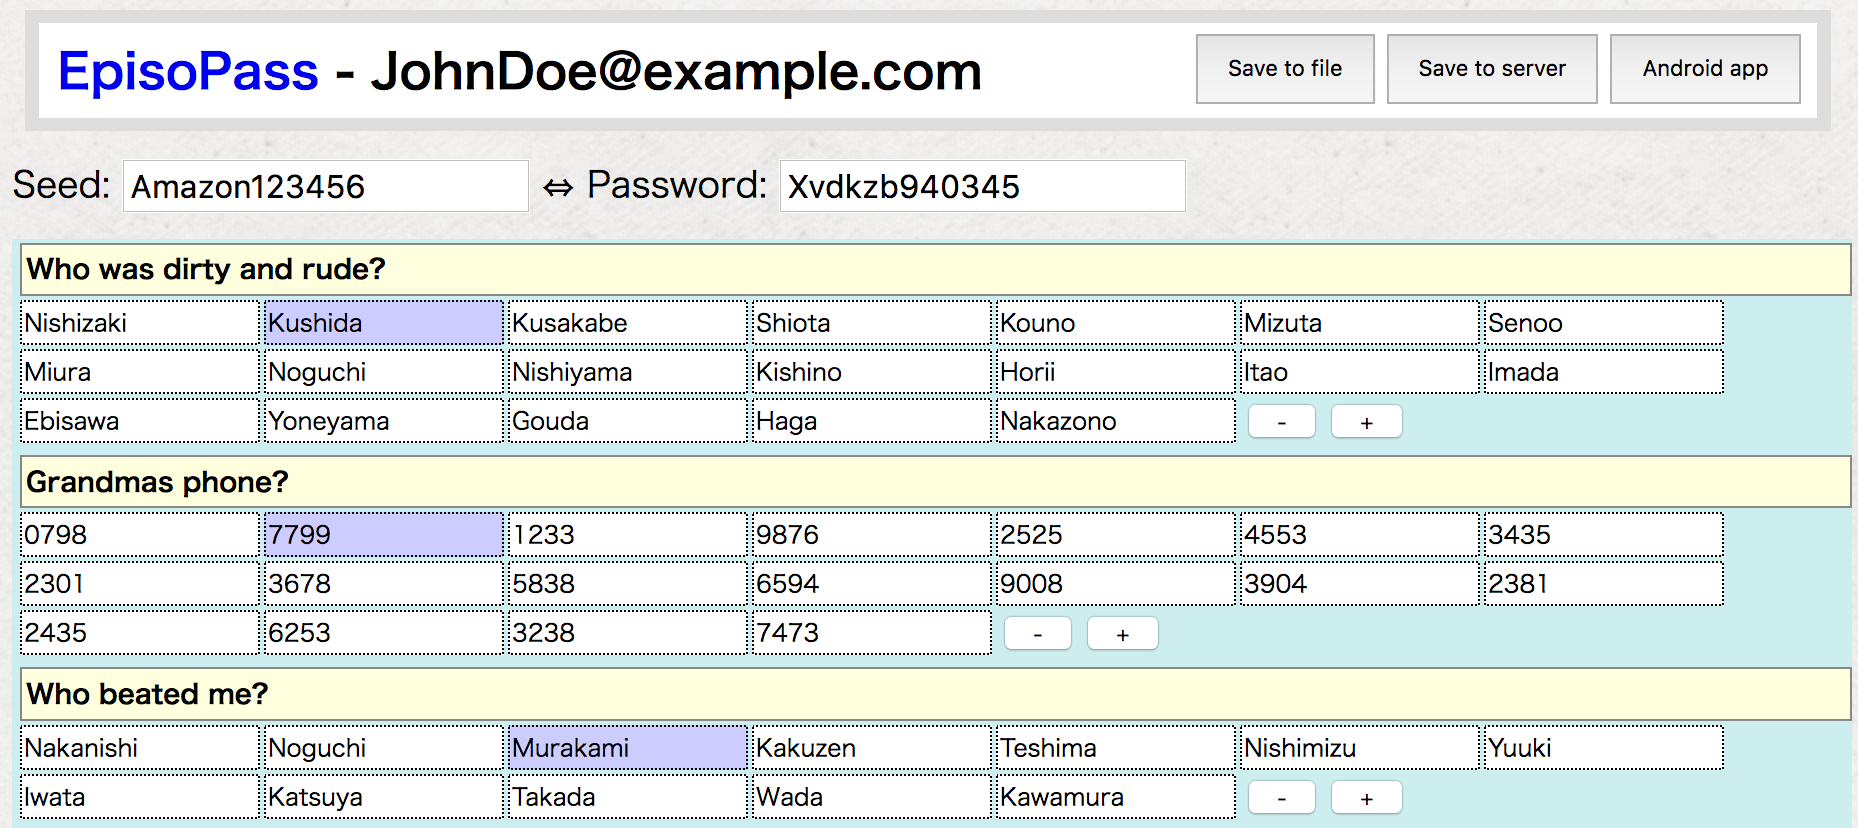
\includegraphics[width=1.0\columnwidth]{figures/8447eaba1ede0f678b3ce6fea63681f3}
\caption{Selecting a different set of answers.}
\label{web11}
\end{figure}

Usability has been considered as a key consideration, and the questions 
and answers in the figures can be edited directly in the browser. They can be
saved on the server by clicking the ``save to server'' button or saved locally
if the user prefers.
While the Q-A data sets are saved, no information about the correct answer or the
generated password is saved on the server. Consequently there is no requirement for the user
to trust the server to keep the data secret.
The Q-A data can be downloaded to the user's local machine in JSON format 
by clicking the ``save to file'' button. To upload the data back to the server, the user
simply drags the JSON file to the EpisoPass page.

When the secret string is changed to ``\textsf{Facebook123456}'',
the generated password changes to ``\textsf{Onjbrppy030937}'',
as shown in Figure \ref{web2}.
In this way, the user can generate different passwords for
different services just by changing the seed string.
Seed strings like ``\textsf{Amazon123456}'' and ``\textsf{Facebook123456}'' are used
in the examples because users can easily remember
for which service the set of seeds and Q-A pairs are used.
Users don't have to remember the seed strings,
just like users don't have to remember the Q-A pairs.

\begin{figure}
  \centering
%  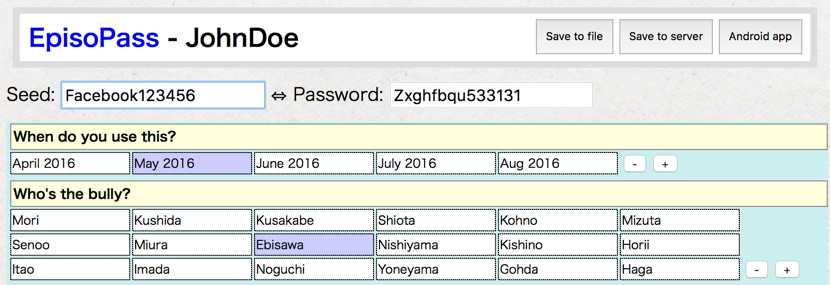
\includegraphics[width=1.0\columnwidth]{figures/0e2820c279afc70520482e0fc53b6ed9}
  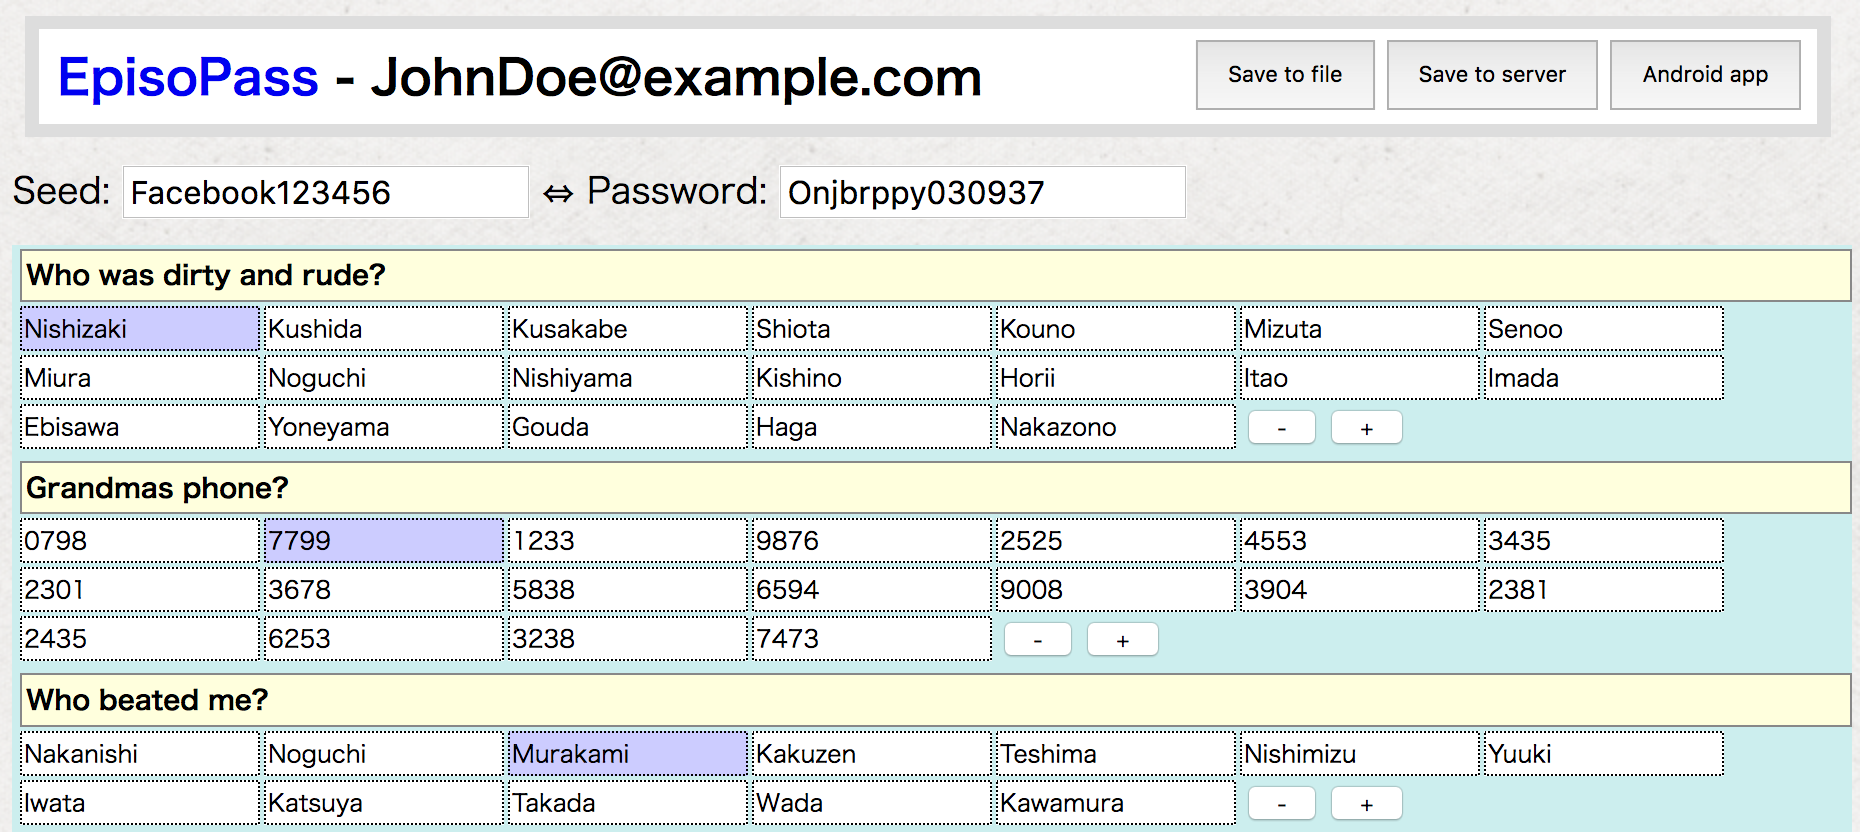
\includegraphics[width=1.0\columnwidth]{figures/ab4517dd593c1cabab5fecef546f7e88}
  \caption{Generating a new password for Facebook.}
  \label{web2}
\end{figure}

Character substitution is performed based on the value
calculated by hashing a concatenation of all the questions and selected answers.
%
For example, if the user selects ``\textbf{\texttt{Ebisawa}}''
as the answer to the question ``\textbf{\texttt{Who's the bully?}}'',
a string including ``\textbf{\texttt{Who's the bully:Ebisawa}}''
is used for calculating the hash value.

The last question in Figure \ref{web1} is not intended as a secret question based on an
episodic memory, but is instead a question
for generating different passwords for different situations.
By providing a question like this, the user can generate completely different passwords
for different months and years, say.

\subsection{Android application}

% \marginnote{Is the Android app generated as a unique app for each
%  user? If so, I think it's worth making this clear.}

If a user prefers not to use the EpisoPass service on the Web, there
is an alternative EpisoPass application for Android which requires no
network connection.  After registering questions and answers on the
EpisoPass service, the user can download an Android application from
the server by clicking the ``Android app'' button at the top of the
page.  The application unique to the user is compiled and built on the
server and contains all of the information needed for the particular
user to generate passwords using the Q-A sets entered.

When the user runs the application and selects the correct answer
to each question, the password will be generated in the same way as
on the site, as shown in Figures \ref{android1} and \ref{android2}.
This can then be copied to the password entry for access
to a particular service.

\begin{figure}
\centering
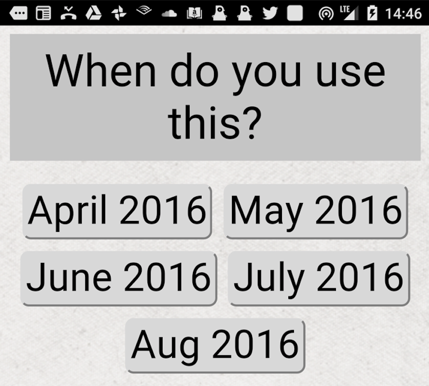
\includegraphics[width=0.4\columnwidth]{figures/429eec261024dc6c85351f51c12f09b4}
\caption{Running EpisoPass on Android.}
\label{android1}
\end{figure}

\begin{figure}
\centering
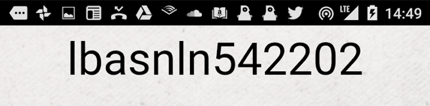
\includegraphics[width=0.4\columnwidth]{figures/ba8f5aeaa935ad63437969f4d746746b}
\caption{After finishing selections.}
\label{android2}
\end{figure}

The calculation is performed on Android without the need for a network connection,
so the user can safely generate passwords without being concerned about an
attacker observing any data transfer.

\subsection{Using the browser extension}
\label{extensionsection}

One of the difficulties of the previous two approaches is that the user 
must re-type or copy the password string into the service's password
field after it's been generated.
This isn't ideally convenient, so we have also developed a browser 
extension that allows EpisoPass to be used directly with the login
page of services on the Web.

\begin{figure}
\centering
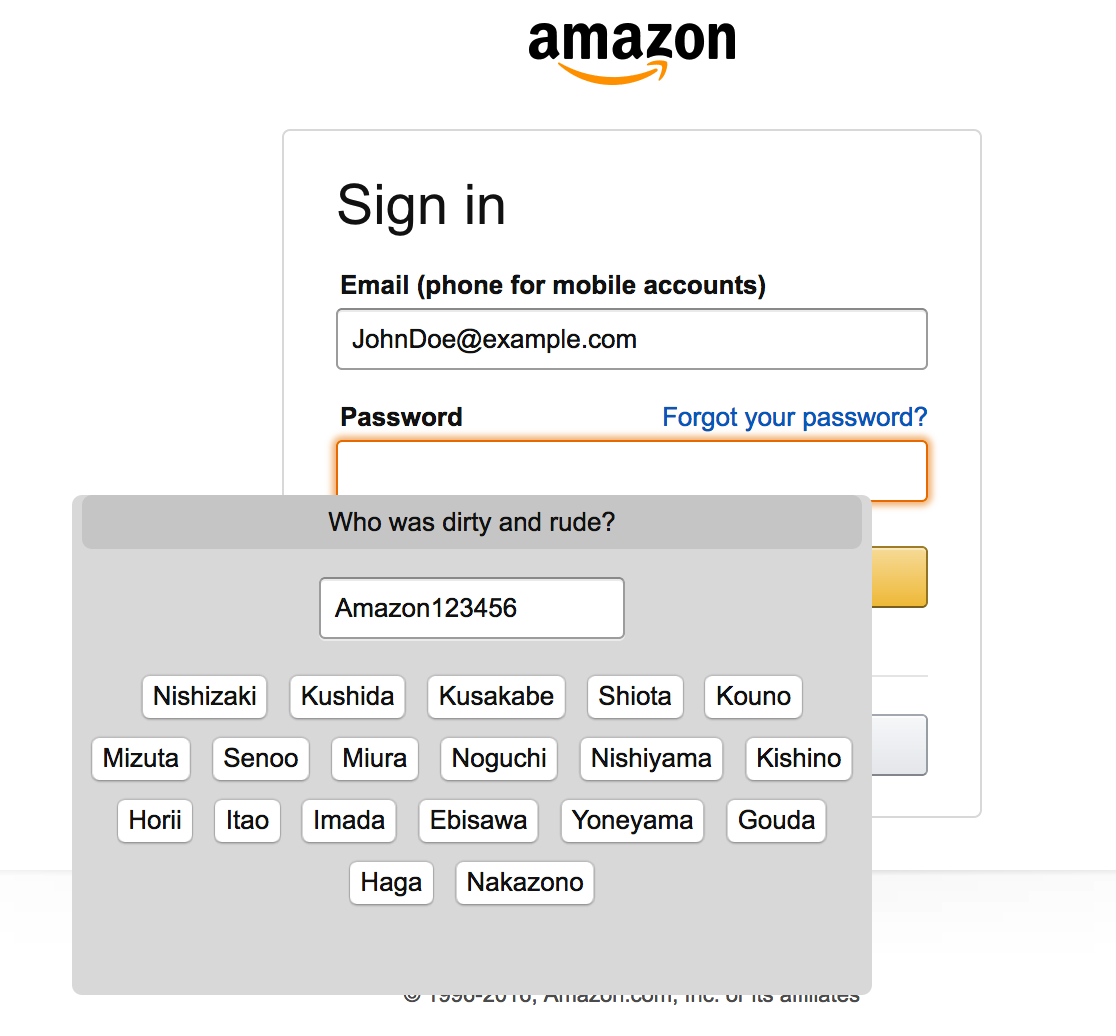
\includegraphics[width=0.8\columnwidth]{figures/aeff16ffcab956e554364e9e5aca8359}
\caption{Using EpisoPass on the login window.}
\label{extension}
\end{figure}

A browser extension is a JavaScript add-on program which runs
on top of existing Web pages.
%
Figure \ref{extension} shows the login page of Amazon.com, with the 
EpisoPass questions automatically overlaid directly onto the page
by the browser extension.
%
When the user accesses the Amazon login page,
the browser extension automatically runs on the page,
acquires the questions and answers from the EpisoPass server,
and displays them using the same style as for the Android application.
%
After answering all of the questions, a password is calculated from the
selected answers and automatically pasted into the password field of the page
by the extension. In this way users can log in to various services just by
answering the questions presented, and without even seeing the password string.
It appears as if the EpisoPass-based authentication is being provided directly
by the services themselves.

\section{Discussion}

In this section, we discuss the advantages and potential disadvantages of using EpisoPass.

\subsection{Recallability of answers}

% David opinion
% \marginnote{The fact that an `old' memory is unlikely to be forgotten
%   is perhaps obvious, but this could be a good place to cite a paper
%   on memory/psychology about this if you're aware of any?}

% Frank:
% I second David's margin note. Can you back this claim--or more
% precisely the implied claim that old episodic memories will be
% unforgettable? (You could argue that no, you only said that IF the
% memory is old, episodic and unforgettable, THEN there's little chance
% to lose the password; you haven't said that IF the memory is old and
% episodic THEN it is unforgettable. Ok, ok, but then the question
% becomes: if I come up with and old and episodic memory, how do I know
% if it's a good one (unforgettable) or one that I will forget later? If
% you answer ``it never happens'' then you must back this claim. If it
% can happen, you should give me a criterion to tell in advance if it
% will, and why I should trust it.

The biggest advantage of using EpisoPass is that
users don't have to remember strong password strings.
%
The seed string and question-answer data is essentially public,
and users of EpisoPass can save them wherever is convenient. They can
then easily generate passwords by running
EpisoPass and answering the questions.
If a question is based on old unforgettable episodic memory,
there is little chance of losing the password for a service
as long as the seed string and questions are available.
If the user's memory is related to an episode that took place 20 years ago, say, and the user clearly
still remembers the episode now, it is unlikely the episode will be forgotten in the future.

\subsection{Selection of seed strings}

% \marginnote{In the comments you mention that ``generating
%   service-specific unique seed string is not trivial''. I think this
%   is worth mentioning in the paper.}

In the previous examples showing the author's EpisoPass questions, a
seed string ``\textsf{Amazon123456}'' was used for Amazon.com, and
``\textsf{Facebook123456}'' was used for Facebook.  Such strings were
chosen because they are easily memorable.  In practice any seed string
could be used as the seeds for the various services, and automatic
generation of seed strings is a possibility, although generating
service-specific unique seed string is not trivial.  For example,
users can use the same username and password both for Amazon.com and
Amazon.co.uk, but not for Amazon.co.jp.

\subsection{Security strength of EpisoPass}

The strength of the generated passwords depends on the number and 
level of secrecy of the questions.
%
There have been many studies on the strength of passwords
\cite{Hayashi:2011:DSP:1978942.1979326,Komanduri:2011:PPM:1978942.1979321}, % What password is strong
but measuring the strength of secret questions is an area where more study is needed.
% \marginnote{I calculate $20^{10} = 10,240,000,000,000$. This is
% considerably more than a billion (closer to 10 thousand billion,
% (US) or 10 million million (UK).}
Using ten secret questions each with twenty answers, where each answer is considered equally likely,
an attacker would need to cover a search space of over ten trillion ($20^{10}$) values to check
every potential combination of answers,
and the entropy of the system is 43.2 ($10 \times \log_2 20$) bits.  % 10.0 * (Math.log(20.0)/Math.log(2.0))
%
This represents roughly the same entropy as using a random 8-character Latin-alphabet
password, for which the entropy is 45.6 bits.
This level is considered to be strong enough for Web services,
where it's not possible to perform online brute-force attacks \cite{Florencio:2007:SWP:1361419.1361429}.

\subsection{Selecting good questions}

The quality of the questions is key to using EpisoPass effectively.
If the episode is shared by someone else,
this other person might easily be able to answer the question and generate the
user's password.
%
The episode related to each question should therefore not be known to any other person,
and the episode should be unforgettable.
%
Finding such episodes seems difficult at first, but our experience
has been that we try to remember such experiences from our personal past,
we can soon recall many trivial episodes which are unforgettable but
nonetheless not important to other people.
%
The following list shows some examples of experiences that we believe make good candidates for
EpisoPass questions.

\begin{itemize}
\item Memories of very minor injuries that nobody would have cared about apart from you.

\item Memories of bad experience such as embarrassing blunders or failures,
especially in the case where it was never admitted to anyone else.

\item Experiences of finding inconsequential but special items which only you are interested in.
\end{itemize}

For example, a question such as
``who hit you when you were six years old?''
is about a trivial experience that most people would never have reason to discuss,
but an experience that may have been unpleasant at the time is hard to forget.

Questions such as ``Which food do you like best?'' should be avoided,
since friends or family might know the user's tastes, thereby allowing 
others to select the correct answer.
Questions related to an episode which the user is proud of should also be
avoided, since this is a something the user might prefer to discuss with others.

We don't usually talk about trivial bad experiences with other people,
but we might boast about good experiences (some might even write blog posts about them).
Similarly our tastes ({\it e.g.\/} favorite foods) might change in the long run.
Using such episodes for questions should therefore be avoided.

\subsection{Creating fake answers}

It can be difficult to provide a large number of false answers to a question like
``what is your favorite sport?''
because the number of possible answers is limited.
%
On the other hand, if the right answer to the question is a name of a place or a person,
generating similar answers is straightforward.
For example, if the answer to the question is ``Colorado'',
we can easily provide fake answers like ``California'', ``Utah'', etc.
because we can use the list of states in the U.S. as possible answers.

In this way, false answers can be easily generated
if it is possible to collect words which belong to the same
category as the right answer.
%
Various methods have been proposed for collecting words in the
same category, mainly for information retrieval tasks
\cite{Huang:2012:LFC:2426725.2426728,BooWa,Wang:2007:LSE:1441428.1442086}. % Boo!Wa!
We can use such systems to provide a list of potential false answers almost automatically.

\subsection{Universality}

Although everyone has to make use of authentication systems, not everyone
is good at handling passwords.
Even experienced computer users have trouble with passwords,
since choosing a good password is unintuitive and remembering complex
passwords is hard.
%
Using EpisoPass, people can use password-based systems without having to invent
techniques for creating and remembering strong passwords. The Q-A configuration step
is a one-time process, after which the system becomes straightforward to use.
%
By integrating EpisoPass into existing password-based services,
people can even use services without noticing that passwords are
required for the service.
%
Our experience of using browser extensions suggests that
this approach offers the most seamless experience.

\subsection{Password requiring frequent updates}

Many services still require users to change passwords periodically in an attempt
to strengthen security.
%
Although this is no longer considered good-practice, since humans struggle to
generate a stream of strong passwords \cite{Schneier:change}, the practice is
still widespread.
%
% A user can generate a new strong password by using a random character generator
% on a password manager, but he might want to old passwords in case some trouble happens.
%
Using EpisoPass, users can provide a date-related question
similar to that shown as the final question in Figure \ref{web1}. This allows
different strong passwords to be generated depending on the answer chosen
for this question. Using this technique, people can easily manage both old and new 
passwords efficiently.

% \subsection{Comparison with challenge-response authentication}
% 
% % 一方、{\SQ}を利用する認証の脆弱性を利用した攻撃が近年問題になっている。
% % {\PW}を忘れたときのために、
% % あらかじめ設定した{\SQ}に答えることによって{\PW}をリセットできるサービスがあり、
% % 「母親の旧姓は?」や「最初に飼ったペットの名前は?」のような
% % 質問に対してユーザが答を登録するようになっている。
% % このような問題は他人が調べたり推測したりすることが容易であるうえに
% % {\SQ}の数は一般的に少なく、
% % {\PW}よりも脆弱だといえる\cite{Rabkin:2008:PKQ:1408664.1408667}。% 銀行20個調べて{\SQ}の弱さを指摘
% 
% In many services, users are advised to define answers to secret questions like
% ``what is your mother's maiden name''
% so that he can log into the service even when he forgets the password.
% This kind of authentication is far less secure than simple password systems,
% since it is fairly easy for attackers to know the right answer.
% The variation of system-provided questions are usually small, and
% such challenge-response systems are considered to be
% insecure\cite{Rabkin:2008:PKQ:1408664.1408667}.
% 
% It would be better if the user can register his own secret questions
% based on his episodic memory.
% However, answers to user-generated challenge questions are more easily
% forgotten or cracked,
% and using simple challenge-responce is not considered to be safe enough
% \cite{Just:2009:PCC:1572532.1572543}\cite{Schechter:2009:NSM:1607723.1608145}.
% %
% Also, in this case,
% the user should register the answer to the system in addition to the question.
% Telling secret facts to service providers is like
% registering raw password string on the server,
% and it is not safe unless the strings are properly hashed and salted on the server.

\subsection{Care for handling secret information}

Users don't have to be very careful about handling questions and answers.
They can even be stored in a public place
given a sufficient number of questions and fake answers are provided.
%
Keeping secrets is a considerable effort for most people (including
the authors), but if the entire set of questions and answers used for EpisoPass
can stored publicly,
handling it becomes straightforward.
This is in contrast to the care needed when handling 
secrets like passwords, secret keys for SSH, {\it etc}. which should
never be copied to or saved in an unsafe place.
The EpisoPass data can be stored as a plain text file wherever is convenient
for the user, since a malicious attacker isn't able to generate
a valid password without also knowing the owner's relevant episodic memories.

% \subsection{Using shared secrets}
% 
% \subsection{Simplicity}
% 
% The algorithm of generating a password (shown in Appendix)
% is fairly simple and
% it can be implemented on any browser JavaScripts or
% applications on smartphones and small devices.
%
% \subsection{Hash function}

\subsection{Risk of server-side password leaks}

If one of the passwords generated by EpisoPass were to be revealed
for some reason, there is a danger that other passwords based on the same questions
might also be revealed.
%
For example, if Twitter is attacked by a hacker and
the password for Twitter (``\textsf{Lbasnln542202}'' in Figure \ref{web1})
is revealed to the attacker,
the attacker could test all answer combinations. If the attacker also had access
to the question and answer strings used, they could then establish the correct 
answers used to generate the password.
Once all the answers to the questions are known,
the attacker can then freely generate all of the user's passwords
generated from the same set of questions.

% \marginnote{It may be helpful to give an indication of how many Q-A sets you think
% would be considered `sufficient' here.}
%
To prevent this, users can prefer saving questions and answers in a secret place or
use sufficient questions to prevent such a brute-force attack from being viable.
The entropy of 12 questions with 30 candidate answers 
is 58.9 ($12 \times \log_2 30$) bits, and this is considered to be safe
enough at this moment.

\subsection{Using images}

% \marginnote{The use of images is nice, but I don't find your argument
%   so convincing here. I have two concerns: first the claim that
%   selecting images will be easy. Second, the example you provide
%   doesn't seem strong, since other people are likely to be able to
%   identify a friend from a photograph.}

Pictures can also be used as EpisoPass questions,
similar to that shown at the bottom of Figure \ref{web1}.
Even if people find it difficult to create good secret questions,
selecting an image from their photo collections
and using it as the question should be straightforward.
For example, if you have an old special picture of a place you visited,
you can use it as the question and use the name of the place
as well as other similar fake place names.
For a secret question, a low-quality photo is better than a
high-quality photo because a low-quality photo
like the one shown in Figure \ref{web1} are not
easily recognizable by other people.

Of course, it's important the photo should have no information related
to the location, especially given how sophisticated
Web-based image searching has become.

\subsection{Password entry time}

Answering to many questions takes much longer time than typing a
remembered password, so people may prefer typing password
rather than using EpisoPass if they have to log in to a service frequently.
The tradeoff betwee security and usability has long been a big issue
of authentication systems \cite{Braz:2007:DTU:1778331.1778344},
but we believe we can approach the best solution by
improving the user interface of answering questions.

% Frank's comment
% 3.11. It takes a rather long time to enter one password!''
% should also be discussed, and may be a killer in some cases. Maybe
% Episopass is good for infrequently used passwords where the penalty of
% a slow login is less relevant.

\section{Related Work}

% 様々なシステムがあるが、エピソード記憶からパスワードを直接生成するものは少ない

As discussed in previous sections,
there have been many attempts to replace password-based authentication systems,
but none of them have yet become as widely deployed as
passwords \cite{Bonneau:ReplacePasswords}.
%
Although cognitive password systems have been an area of study for 
many years \cite{Lazar2011,Zviran:1990:UAC:100512.100538},
implementations up to now have all been intended as replacements 
to password-based systems, requiring support from the services involved.
As far as the authors are aware, ours is the first password-generation systems to be
based on cognitive authentication.

% 普段の行動を質問に利用する[][]
% \ref{Dandapat:2015:AYD:2702123.2702457} % 日常行動からパスワード作るActivePass
% これはパスワードを作るのか
% \ref{Das:2013:ECE:2493432.2493453} % スマホの利用状況を認証に使う
% \ref{conf/percom/GuptaWRLGB12} % スマホの利用状況を認証に使う
% これはEpisodicMemoryと関係ないなぁ

The idea of using episodic memories for authentication is also not new.
In fact, using episodic memories for selecting passwords
has generally been recommended,
and many current computer users are probably using password that are
in some way informally related to their episodic memories.

Recent work has considered the use of mobile devices for authentication,
in particular harnessing the fact that a mobile device captures large quantities
of personal information. A mobile device may therefore be able to identify
its user based on their previous behavior; events which only the user would be able to recall \cite{Dandapat:2015:AYD:2702123.2702457,Das:2013:ECE:2493432.2493453,GuptaWRLGB12}%
.
For example, if a user can answer questions such as
``who did you call last night?'' correctly, the authentication will succeed.
Using mobile or wearable devices for authentication will become more usable
in the future,
but in order for this to work effectively users must be able to remember potentially
arbitrary behavior over the long-term. This may be a challenge for many people, and the 
benefit of EpisoPass in comparison is that the user is able to select memories that they
know to be memorable, rather than having their mobile device choose them arbitrarily.

Various types of image-based authentication systems have been proposed recently
\cite{Biddle:2012:GPL:2333112.2333114,GraphicalPasswords},
based on the realisation that images are easier to remember than text
given they are usually more directly linked to episodic memories.
However, some image-based authentication systems request
users to remember new secrets related to the images instead of
using the users' old episodic memories.
This turns out to be not much easier to remember than passwords.
%
% \marginnote{This statement seems to contradict what you said above
%   about it being easy to find images. Probably the phrasing just needs
%   a bit of refinement.}

Image-based authentication based on episodic memories might work
if users can prepare many images 
that are tightly linked to their episodic memories.
However, finding such images is usually not straightforward, and
image-only authentication systems are unlikely to become popular
until simple and effective techniques for doing so have been developed.

Even when a new ideal authentication method is invented,
replacing all the password-based systems will still be a lengthy process. 
Password managers will therefore remain important until this hypothetical
ideal solution has become ubiquitous.
In the age of password-based authentication,
using password managers seems to be the only way to tackle
the problem of passwords.
%
While most of the password managers only remember passwords given by the user,
generating passwords with a password manager is a new approach for
handling password-based systems.
Just like EpisoPass generates passwords,
Versipass \cite{Stobert:2014:PMD:2683467.2683471} %Versipass 画像のヒントからパスワード生成 % A Password Manager that Doesn’t Remember
helps the user to generate password strings
using ``visual cues'' from an arbitrary image.
Instead of directly using images for authentication,
users use the system to generate a password string with the help of
the image shown to the user.

% 強いパスワードを作るシステム
%   ランダムに生成するサイトが沢山ある
% 
% 強いパスワードを覚えるための工夫 ★
%   Bonneau
% 
% パスワードに関する全情報を公開してどこかに置いておける
%   ググれるかもしれない
%   紛失する可能性が少ない
%

\section{Experiences}

EpisoPass has been used by the authors for more than three years
for various services including Twitter, Facebook, Amazon, Skype, {\it etc}.
% Since passwords for these services are remembered on the browser,
% EpisoPass is used only once in one week at most.
%
Before using EpisoPass, managing multiple passwords was a significant challenge
for the authors. We now have all the information for generating passwords 
stored in the cloud and no problems have arisen during this period.
%
Since the introduction of our browser extension, visiting the EpisoPass 
service has now become unnecessary, making authentication to the various
services even easier.

The EpisoPass service is available via the Website and the source code is
available on GitHub\footnote{
  (url removed for double-blind review)
  % \url{https://EpisoPass.com/},
  % \url{https://github.com/masui/EpisoPass}
}. EpisoPass currently has only a small user-base, one major
reason being that most people cannot fully understand the
idea behind EpisoPass, and may not trust it without the 
support of a well-known IT company.
% nor supported by famous computer users.
Another reason is that it's difficult for users to
assess the security of EpisoPass.
Since the intention is for the questions and answers to be obvious
to those that know them (but not to others), users may lack
confidence in their answers being unknown to others.
Any authentication system expecting widespread use must take
such psychological issues seriously, and we hope to address 
such issues in future work.

\section{Conclusion}

We introduced a password management system {\it EpisoPass\/}
that converts a seed string into a password using the user's
episodic memories. These memories are represented as a set of questions and answers
which can be solved only by the user in order to generate a site-specific password.
%
Using EpisoPass with well-defined questions and answers,
a user can always retrieve a service's passwords without worrying about
having to remember any secret information, other than the episodic memories
that have been chosen specifically to be easy to recall.
%
In future work we hope to integrate the system with more existing password-based
services, and ultimately aim to address the problems
derived from password-based authentication.

% {\EM}に結びついた{\SQ}を利用して{\PW}を生成/管理できるシステム{\EP}を提案した。
% {\EP}は単純な原理にもとづいており柔軟な利用形態が可能であり、
% 強力な{\SQ}を用意することにより
% 秘密情報を全く覚えることなく安全な認証を行なうことができる。
% %
% 強力な{\SQ}を作成して安全に運用が可能かどうかを長期的に評価したいと考えている。
%
%欠点:
%なぞなぞを考えるのがめんどくさい
%安全になぞなぞを扱うのが面倒
%  ネットなしで運用したりとか
%運用を間違うと思わぬところで回答がバレる可能性がある
%
% {\EP}は\textsf{http://Episopass.com/}で運用しており、
% ソースはGitHubで公開している\footnote{
%   \textsf{http://GitHub.com/masui/EpisoPass}
% }。

\subsection*{Note.}

This paper is largely a translation of a 2013 paper published by the
author in Japanese \cite{WISS2013}. This is the first time that the
work is presented to an international audience in English.
Additionally, in the intervening three years the author has
developed the browser extension described in section \ref{extensionsection}.

%%%%%%%%%%%%%%%%%%%%%%%%%%%%%%%%%%%%%%%%%%%%%%%%%%%%%%%%%%%%%%%%%%%%%%%%%%%%%%%%%%%%

% \subsection{Citations}

% \marginnote{I've added some text in about the grant. Please change it
%   as you see fit of course. I'm afraid I don't know the grant number
%   so have left a gap; ideally this should be added in too.}

% \subsubsection*{Acknowledgments.}
% This paper was written while on
% sabbatical at the University of Cambridge, hosted by Frank Stajano and
% the Pico group, and supported by EPSRC grant number
% EPSRC IRIS grant EP/M019055/1 on  ``Future Authentication Systems''.

\bibliographystyle{splncs03}
\bibliography{paper}

\end{document}

